% LaTeX/AMS-LaTeX

\documentclass[a4paper,11pt]{book}
\usepackage[utf8]{inputenc}
%%\usepackage[portuges]{babel}

\usepackage{amssymb}
\usepackage{amsmath}
\usepackage[dvips]{graphicx}

\begin{document}

\chapter{Primeiros passos no Perl}

\noindent Virtualmente todas linguagens de programa\c{c}\~ao possuem algumas coisas em comum. Os conceitos fundamentais de programa\c{c}\~ao s\~ao os mesmos, n\~ao importa que linguagem voc\^e est\'a utilizando. Neste cap\'itulo vamos investigar o que voc\^e precisa saber antes de iniciar a codifica\c{c}\~ao do programa. Por exemplo:

\begin{itemize}

 \item O que \'e a programa\c{c}\~ao afinal? 

 \item O que significa programar?

 \item O que acontece com o programa que escrevemos?

 \item Como estruturamos os programas e como o constru\'imos de maneira a torna-los de f\'acil compreens\~ao?

 \item Como os computadores v\^e as letras e os n\'umeros?

 \item Como podemos encontrar e eliminar erros nos nossos programas? 

\end{itemize}

\noindent Claro que veremos isto da perspectiva do Perl, e vamos analisar alguns programas b\'asico em Perl, ver como eles foram constru\'idos e o que fazem. Ao final deste cap\'itulo voc\^e ser\'a convidado a escrever o teu pr\'oprio programa.

\section{Linguagens de programa\c{c}\~ao}

\noindent A primeira pergunta que eu suponho que realmente devemos fazer quando iniciamos o aprendizado sobre programa\c{c}\~ao \'e: "O que \'e programa\c{c}\~ao?". Isso pode soar particularmente filos\'ofico, mas a resposta \'e f\'acil. Programa\c{c}\~ao \'e dizer a um computador o que voc\^e quer que ele fa\c{c}a. O \'unico truque, ent\~ao, \'e ter certeza de que o programa \'e escrito de uma forma que o computador possa entender, e para isso, temos de escrever numa l\'{\i}ngua que podemos compreender - uma linguagem de programa\c{c}\~ao, como Perl.

\noindent 

\noindent Escrever um programa n\~ao requer habilidades especiais, mas \'e necess\'ario um modo particular de pensar. Quando damos instru\c{c}\~oes para seres humanos, assumimos algumas como certo.

\begin{itemize}

 \item Humanos questionam quando n\~ao compreendem as instru\c{c}\~oes.

 \item Quebramos tarefas complexas em sub-tarefas.

 \item Podemos tra\c{c}ar paralelos entre a tarefa atual e aqueles que conclu\'{\i}mos no passado.

 \item Talvez mais importante ainda, n\'os podemos aprender a partir de manifesta\c{c}\~oes e de nossos pr\'oprios erros.

\end{itemize} 

\noindent Os computadores ainda n\~ao podem fazer qualquer uma dessas coisas muito bem – e ainda \'e muito mais f\'acil de explicar a algu\'em como amarrar seus sapatos do que corrigir o rel\'ogio no v\'{\i}deo cassete.

\noindent 

\noindent A coisa mais importante que você precisa ter em mente, porém, é que você não será capaz de expressar uma tarefa para um computador, se você não pode exprimi-la a si mesmo. Programação de computador não tem espaço para especificações vagas. Se você quiser escrever um programa para, por exemplo, remover arquivos inúteis do seu computador, você precisa ser capaz de explicar a si mesmo como determinar o que é um arquivo é inútil ou não. Você precisa analisar e detalhar os processos necessários para realizar a tarefa para si mesmo: Você poderia excluir um arquivo que não tenha sido acessado por um longo tempo? Quanto tempo, mais precisamente? Apagar o arquivo imediatamente, ou examiná-lo? Se você examiná-lo, quanto dele vai examinar? E o que você examinará?

\noindent 

\noindent O primeiro passo em programação é parar de pensar em “quero um programa que remove arquivos inúteis”, para “eu quero um programa que verifique cada arquivo no computador e remova os criados a mais de seis meses e que não contenha qualquer uma das palavras 'Simon', 'Perl' ou 'importantes' nas cincos primeiras linhas”. Em outras palavras, você tem de especificar a sua tarefa com precisão..

\noindent 

\noindent Quando você for capaz de restruturar a sua pergunta, é necessário traduzi-la para a linguagem de programação que você está utilizando. Infelizmente, a linguagem de programação não possui uma relação equivalente direta para o que você está tentando dizer. Então, você terá que desenvolver as tuas atividades utilizando o que a linguagem tem a lhe oferecer, o quê significará que você precisará detalhar (especificar) mais ainda a tua tarefa. Por exemplo, não existe uma maneira de dizer "que não contenha qualquer uma destas palavras nas cincos primeiras linhas" em Perl. No entanto, existe uma maneira de dizer "se uma linha contém a palavra", uma maneira de dizer "buscar outra linha", e "faça isso cinco vezes". A programação é a arte de colocar os elementos juntos para fazer o que você deseja.

\noindent 

\noindent Existe tantas coisas para você fazer – mas o que computador faz? Depois termos especificado as tarefas em nossa linguagem de programação, o computador pega nossas instruções e executa-as. Chamamos isto de \textbf{'rodando'} ou \textbf{'executando'} o programa. Normalmente, vamos escrever as instruções em um arquivo, utilizando um editor de texto normal; mas se temos um programa muito pequeno, podemos digitá-lo diretamente na linha de comando. De qualquer forma, as instruções que damos ao computador - no nosso caso, escrito em Perl - são coletivamente chamado de \textbf{código fonte} (ou, por vezes, apenas \textbf{código} ou \textbf{code}) para nosso programa.

\section{Interpretado vs Código Compilado}

\noindent O que exatamente o computador faz com o nosso código fonte, então? Tradicionalmente, havia duas formas de descrever o que a linguagem de computador fazia com o código fonte: Pode-se dizer que foram \textbf{compilados}, ou \textbf{interpretados}.

\noindent 

\noindent Uma linguagem interpretada, como o Basic, precisa de outro programa chamado \textbf{interpretador} para processar o código fonte cada vez que você deseja executar o programa. A tradução do código fonte para a linguagem de máquina é demorado. Nós chamamos de linguagem de baixo nível, ou \textbf{código de computador}, porque é linguagem para a máquinas ler, já o \textbf{código fonte} é para os seres humanos. Enquanto que o código fonte parece com o Inglês, por exemplo, \texttt{("do\_this() if \$that")}, já o código de máquina parece muito mais com algo como por exemplo, \texttt{"4576616E67656C6961"}, e esta é a versão legível! O código de máquina produzida depende do processador do computador e do sistema operacional executado, a tradução seria muito diferente de um computador x86 executando o Windows NT, em comparação com um SUN ou Digital executando Unix.

\noindent 

\noindent Por outro lado, uma linguagem compilada, como o C, utiliza um compilador que faz todo esse processamento de uma só vez antes do código ser executado. Depois disso, você pode executar o código máquina diretamente, sem precisar mas do compilador. Porque você não precisa processar o código fonte cada vez que você execute-o, código compilado normalmente será executado rápido do que um equivalente interpretado. Você também pode dar o código compilado para pessoas que não têm um compilador. Isto também prevenirá que outras pessoas leem o seu código fonte - útil se você estiver usando um algoritmo proprietário ou se o seu código é particularmente embaraçoso/vergonhoso. No entanto, porque você está distribuindo código máquina que nem todos os tipos de computadores possam compreender, isto não é necessariamente portáteis.

\noindent 

\noindent Recentes linguagens têm confundindo a distinção compilado/interpretado. Java e Perl, ambas linguagem da classe  de "byte-compilados", são particularmente responsáveis pela confusão. No caso do Perl, onde o interpretador (que sempre chamamos de \textbf{perl} com "p" minúsculo) lê o seu código fonte, e o compila inteiro de uma vez. No entanto, em vez de compilar para o código da máquina que em está executando, ele compila em um código especial para uma \textbf{máquina virtual (virtual machine)} de um computador fictício. A "máquina virtual" do Java é muito parecido com o processador de um computador normal, em relação ao que pode ser feito, e pessoas têm tentado construir processadores que possa conversar código da máquina virtual Java "nativamente". Em comparação, a máquina virtual do Perl não é muito semelhante a qualquer processador de  computador existente e por isto menos susceptível de ser construído.

\noindent 

\noindent Uma vez que temos esse código de máquina, o que chamamos \textbf{bytecode}, você pode fazer uma série de coisas com ele. 

\noindent Você pode:

\begin{itemize}

 \item Armazena-lo agora para ser executado depois.

 \item Traduzi-lo para o código nativo do seu computador, e executá-lo imediatamente.

 \item Executá-lo através de um programa que finge ser a máquina virtual e através do processamento do bytecode, executa as ações apropriadas.

\end{itemize}

\noindent Nós não fazemos o primeiro item em Perl, embora Java o faz. O "Perl compilador" tenta fazer o segundo, mas é uma tarefa muito complicada, e ainda não está completo. Normalmente, porém, fazemos o terceiro, e assim que o perl terminar de compilar o código fonte em bytecodes, depois assume o papel de interpretador, traduzindo o código da máquina virtual para o código verdadeiro. Daí Perl não é uma linguagem  estritamente compilada ou interpretada.

\noindent 

\noindent Algumas pessoas vão dizer é que Perl é uma linguagem de "script", com a conotação de que é uma linguagem interpretada. Como vimos, isso não é realmente verdade. No entanto, esteja ciente de que você pode ouvir a palavra "script" com a intenção de "programa".

\section{Bibliotecas, Módulos e Pacotes}

\noindent Um monte de gente usa Perl. Uma consequência disto é que, sem surpresa, um monte de código Perl tem sido escrito. De facto, uma grande parte do código Perl que você necessitará escrever provavelmente já tenha sido escrito antes. Para evitar perda de tempo reinventando a roda, programadores Perl empacotam seus códigos reutilizáveis e os distribuí, principalmente no CPAN - a Comprehensive Perl Archive Network - que você pode encontrar on-line em http://www.perl.com/CPAN/.

\noindent 

A maior parte do CPAN é composto por \textbf{módulos} Perl. Um módulo é um arquivo ou um conjunto de arquivos que permite realizar uma tarefa. Existe módulo para que formatar texto em parágrafos, para desenhar gráficos, e até mesmo efetuar o download e instalar outros módulos. Seus programas podem utilizar estes módulos e adquirir suas funcionalidades. Posteriormente, iremos dedicar a totalidade do Capítulo 10 para usar, instalar, e escrever módulos.

\noindent 

\noindent Intimamente ligada à ideia de um módulo é o conceito de \textbf{pacote}, que é outra maneira de dividir um programa. Ao utilizar pacotes, você pode ter certeza que o que você faz em uma seção do seu programa não afeta outra seção. Considerando que um módulo trabalha com um arquivo ou grupo de arquivos no disco, um pacote é apenas parte do código-fonte. Um único arquivo, por exemplo, pode conter vários pacotes Inversamente, um pacote pode ser repartido por vários arquivos. Um módulo normalmente vive em sua própria embalagem, isolando o código que você escreve fora de interferência. Novamente, vamos chegar a isso mais tarde no Capítulo 10.

\noindent 

\noindent Every Perl installation comes with a collection of 'core modules'. The \textbf{core}, unsurprisingly, is the collective term for the files that are installed with your Perl distribution. At times, they're also referred to as the 'module library', although this could cause confusion if you intend to look back at older Perl code: 'library files' were used in Perl in versions 4 and earlier until replaced by modules in Perl 5. They are the same thing -- pieces of code that you can use in your program to do a job that's been done before. However, they didn't have a package of their own, and so they put themselves in the same package as the rest of your program. It's also fairly simple to spot which file is a library and which is a module -- the extension for a library file is usually .pl, whereas the extension for a module is .pm.

\noindent 

\noindent The result of this is that the module library contains library files as well as modules, and so it's hopelessly unclear what 'library' refers to any more. From now on, if we talk about a 'library', we're referring to the collection of files distributed with Perl, rather than Perl 4 library files; we won't be doing any work with library files (while library files have more or less been replaced by modules, they can still be useful) but will use the new-style modules instead.

\noindent 

\section{Why Is Perl Such A Great Language?}

\noindent Perl is in use on millions of computers, and it's one of the fastest-growing programming languages available. Why is this? We've already seen a number of reasons for this in the introduction, but I think it's worth restating them briefly here.

\subsection{It's Really Easy}

\noindent Perl is not a difficult language to learn. It's a language that tries to shape itself around the way humans think about problems and provides nothing contrary to their expectations. Perls' designers believe that Perl is a populist language -- and not just for the mathematicians and computer scientists of this world.

\noindent I know plenty of people with scientific and non-scientific backgrounds alike who successfully use Perl.

\subsection{Flexibility Is Our Watchword}

\noindent Perl doesn't want you to see things the way the computer does -- that's not what it's for. Instead, Perl allows you to develop your personal approach to programming. It doesn't say that there's one right or wrong way to get a job done. In fact, it's quite the opposite -- the Perl motto is "There's more than one way to do it", and Perl allows you to program whichever way makes most sense to you.

\subsection{Perl on the Web}

\noindent Perl's influence is not felt among the shell scripters of the world alone. Not only can it be used for rooting around in directories or renaming files, it also has massive importance in the world of \textbf{CGI} \textbf{scripting }out on the World Wide Web. You'll find lots of Perl automating communication between servers and browsers world-wide and in more than one form. \textbf{Perlscript} is a (relatively  new) derivation of Perl into a  proper scripting language that can run both client-  and server-side  web routines,  just as Javascript can.  As  we've  said  however,  Perl's  main  function  on  the web  is  as  a  way to script CGI routines.

\noindent 

\noindent For a while, CGI was the standard way for a web server to communicate with other programs on the server, allowing the programs to do the hard work of generating content in a web page while the server dedicated itself to pass that content onto browsers as fast as it could. Of course, web pages are completely text-based and, thanks to its excellent text-handling abilities, PerlCGI set the standard for web server automation in the past. It's CGI (and Perl) that we have to thank for the wonderfully dynamic web pages we have become accustomed to on the Internet.

\noindent 

\noindent Later on in Chapter 12, we will explore the world of CGI in some detail, and among other things, we'll also see how to write CGI scripts using Perl. For the moment, however, let's get back to learning about Perl itself. If you would like to take a look, more information on PerlCGI and PerlScript is available at www.fastnetltd.ndirect.co.uk/Perl/index.html.

\noindent 

\subsection{The Open Source Effort}

\noindent 

\noindent Perl is free. It belongs to the world. It's Larry Wall's creation language, of course, but anyone in the world  can download it, use it, copy it, and help make improvements. Roughly six hundred people are named in the  changes files for assisting in the evolution from Perl 4.0 to Perl 5.0 to Perl 5.6, and that doesn't include the people who took the time to fill in helpful bug reports and help us fix the problems they had.

\noindent 

\noindent When I say 'anyone can help', I don't mean anyone who can understand the whole of the Perl source code. Of course, people who can knuckle down and attack the source files are useful, but equally useful work is done by the army of volunteers who offer their services as testers, documenters, proofreaders and so on. Anyone who can take the time to check the spelling or grammar of some of the core documentation can help, as can anyone who can think of a new way of explaining a concept, or anyone who can come up with a more helpful example for a function.

\noindent 

\noindent Perl development  is done  in the  open,  on  the  \textbf{perl5-porters  }mailing  list.  The perlbug program, shipped with Perl,  can be used  to  report  problems  to  the  list,  but it's  a  good idea  to  check  to make sure that it really is a problem and that it isn't fixed in a later or development release of Perl.

\noindent 

\subsection{Developers Releases and Topaz}

\noindent Perl is a living language, and it continues to evolve. The development happens on two fronts:

\noindent 

\noindent Stable releases of Perl, intended for the general public, have a version number x.y.z  where  z  is less than 50. Currently, we're at 5.6.0; the next major stable release is going to be 5.8.0. Cases where z is more than 0 are maintenance releases issued to fix any overwhelming bugs. This happens extremelyc infrequently. For example, the 5.5 series had three maintenance releases in approximately one year of service.

\noindent 

\noindent Meanwhile between stable releases, the porters work on the development track, (where y is odd). Whenc5.6.0 was released, work began on 5.7.0 (the development track) to eventually become 5.8.0. Naturally, releases on the development track happen much more frequently than those on the stable track, but don't think that you should be using a development Perl to get the latest and greatest features or just because your stable version of last year seems old in comparison to the bright and shiny Perl released last week. No guarantees whatsoever are made about a development release of Perl.

\noindent 

\noindent Releases are coordinated by a 'patch pumpkin holder', or 'pumpking' -- a quality controller who, with help from Larry, decides which contributions make the grade and when and bears the heavy responsibility of releasing a new Perl. He or she maintains the most current and official source to Perl, which they sometimes make available to the public: Gurusamy Sarathy is the current pumpkin, and keeps the very latest Perl at \texttt{ftp://ftp.linux.activestate.com/pub/staff/gsar/APC/perl-current/}.

\noindent 

\textit{Why a pumpkin? To allow people to work on various areas of Perl at the same time and to avoid two people changing the same area in different ways, one person has to take responsibility for bits of development, and all changes are to go through them. Hence, the person who has the patch pumpkin is the only person who is allowed to make the change. Chip Salzenburg explains:}

\noindent \textit{'David Croy once told me once that at a previous job, there was one tape drive and multiple systems that used it for backups. But instead of some high-tech exclusion software, they used a low-tech method to prevent multiple simultaneous backups: a stuffed pumpkin. No one was allowed to make backups unless they had the "backup pumpkin".'}

\noindent 

\noindent So what development happens? As well as bug fixes, the main thrust of development is to allow Perl to build more easily on a wider range of computers and to make better use of what the operating system and the hardware provides for example support for 64-bit processors. (The Perl compiler, mentioned above, is steadily getting more useful but still has a way to go.) There's also a range of optimizations to be done, to make Perl faster and more efficient, and work progresses to provide more helpful and more accurate documentation. Finally, there are a few enhancements to Perl syntax that are being debated -- the 'Todo' file in the Perl source kit explains what's currently on the table.

\noindent 

\noindent The other line of development that's going on is the \textbf{Topaz }project, led by Chip Salzenburg, an attempt to rewrite the entirety of Perl in C++. Compared to the main development track, this is going slowly but steadily. Topaz is by no means ready for use; currently, it can merely emulate some of the Perl internals; there is no interpreter or compiler yet and probably will not be for some time. However, it's expected that Topaz development will speed up in the near future. The homepage of the Topaz project is \texttt{http://topaz.sourceforge.net/}.

\subsection{Our First Perl Program}

\noindent I'm assuming that by now you've got a copy of Perl installed on your machine after following the instructions in the introduction. If so, you're ready to go. If not, go back and follow the instructions. What we'll do now is set up a directory for all the examples we'll use in the rest of the book and write our first Perl program.

\noindent 

\noindent Here's what it'll look like:

\noindent 

\noindent \texttt{\#!/usr/bin/perl -w}
\noindent \texttt{print "Hello, world.\textbackslash n";}

\noindent 

\noindent The 'Hello World' example is the traditional incantation to the programming gods and will ensure your quick mastery of the language, so please make sure you actually do this exercise, instead of just reading about it.

\noindent 

\noindent Before we go any further however, a quick note on editors. Perl source code is just plain text and should be written with a plain text editor, rather than a word processor. If you're using Windows, you really will want to investigate getting hold of a good programmer's editor. Notepad may be fine for this example, despite its annoying tendency to want to rename file extensions to .plx.txt for you, but I wouldn't recommend its use beyond that. WordPad also renames file extensions for you, and additionally, you must remember to save as plain text, not Word format. Edit was bearable, but no longer ships with Windows versions after 95.

\noindent 

\noindent A decent editor will help you with bracket matching indentation and may even use different colors to point out different parts of your code. You will almost certainly want to view and edit your code in a fixed-width font. The usual Unix editors, vi, emacs, and so on are perfectly suitable, and versions ('ports') of these are available for Windows -- I personally use a port of vim a vi-like editor -- available at http://shareware.cnet.com --, when programming on Windows. Right then, back to the code.

\noindent \textit{If You are a Windows User}

\noindent 1. Open Windows Explorer. Left click on the icon for your C: drive and choose \underbar{N}ew \textbar \underbar{F}older from the \underbar{F}ile menu.

\noindent 2. Give the folder the name 'BegPerl' and press Return.

\noindent 3. Open Notepad, which you'll find in the Programs \textbar Accessories menu under the Start button, and type in the two lines of code as shown above.

\noindent 4. Choose Save As from the File menu and change the menu option in Save as type to All Files (*.*). Find your BegPerl folder, and save the file as hello1.plx. The caption box should

\noindent 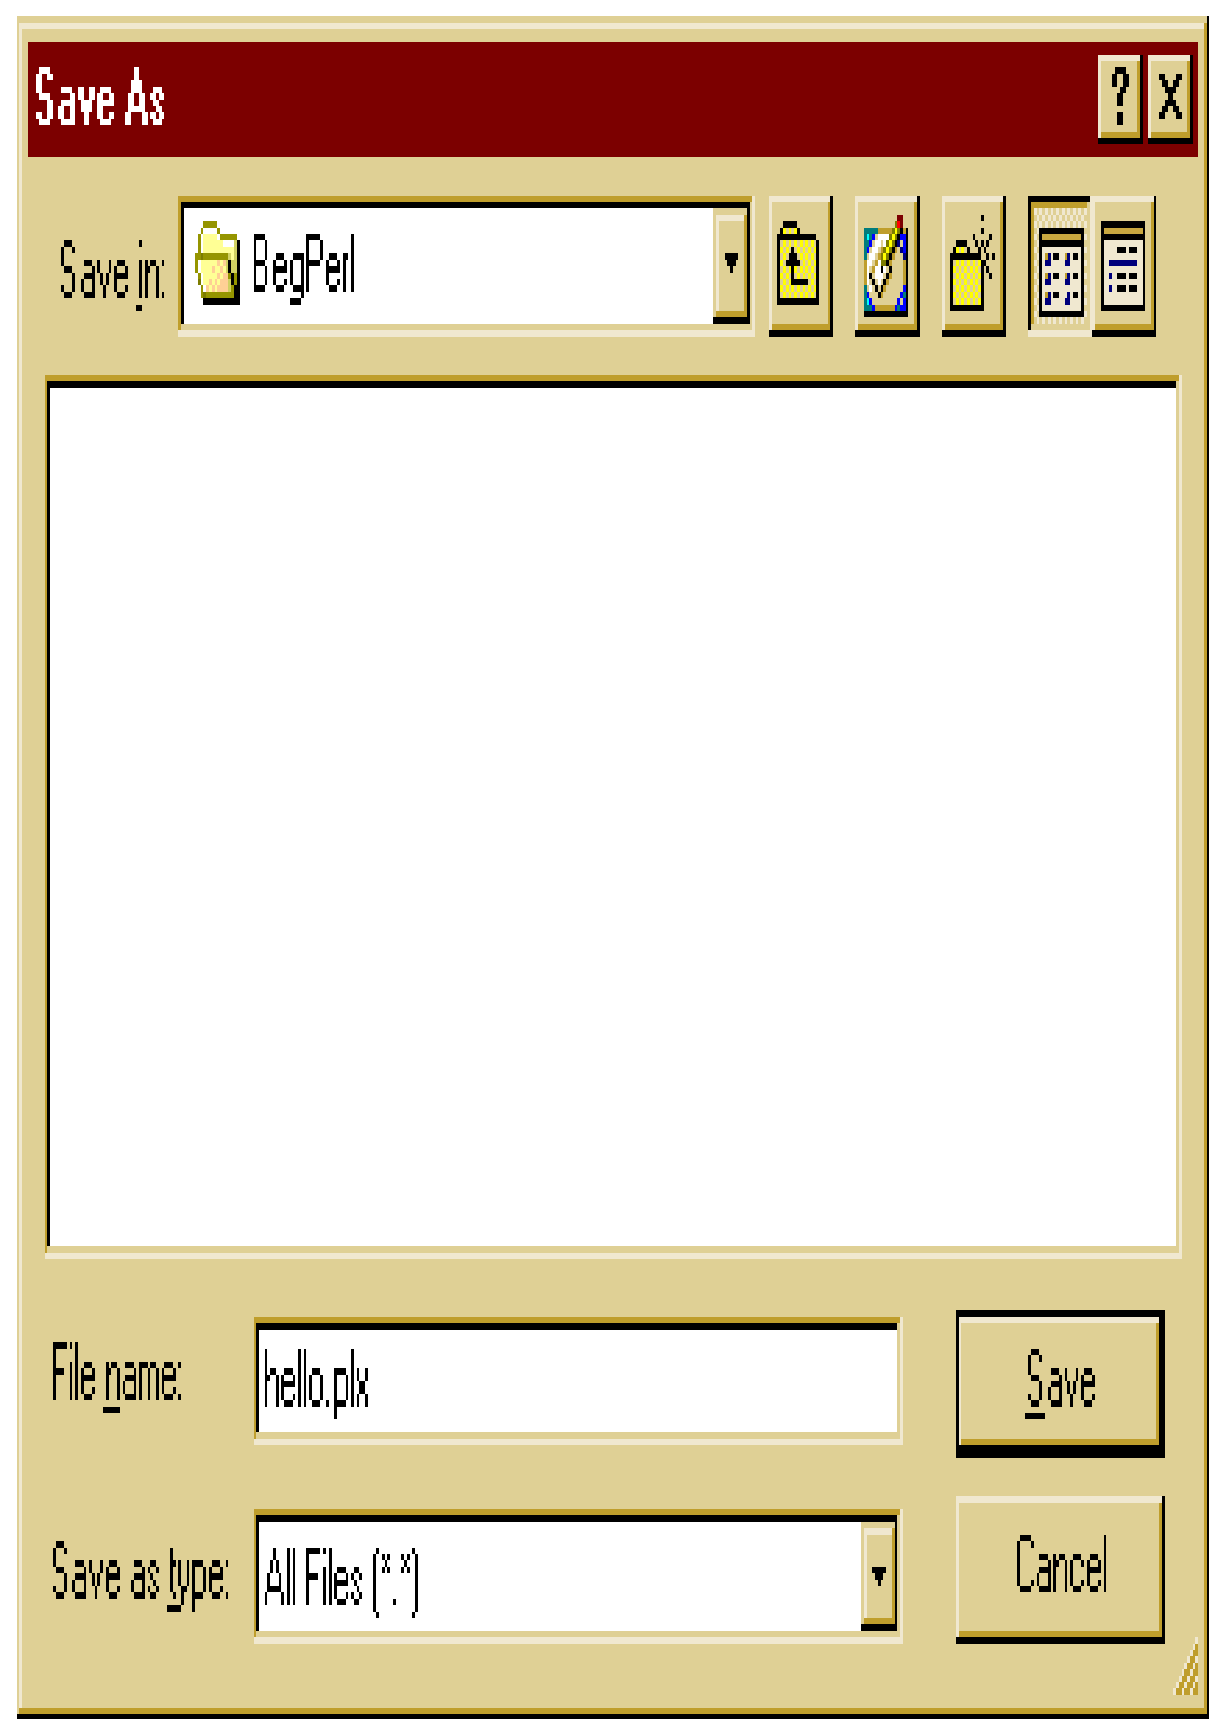
\includegraphics[bb=0mm 0mm 208mm 296mm, width=70.2mm, height=43.6mm, viewport=3mm 4mm 205mm 292mm]{image5.ps}look this.

\noindent 

\noindent 5. Click Save and then exit Notepad.

\noindent 6. It's possible that Notepad will have renamed your file hello1.plx.txt, so in Windows Explorer, go to the BegPerl folder. If it has been renamed, right-click on the file and select Rename. Rename the file back to hello1.plx

\noindent 7. The icon should change to a picture of a pearl 
\includegraphics[bb=0mm 0mm 208mm 296mm, width=3.7mm, height=3.2mm, viewport=3mm 4mm 205mm 292mm]{image6.ps} -- double click on it, and you'll see a window appear briefly and disappear before you have time to read it. This is your first lesson about clicking on Perl programs -- a window will open to run them in, run them, and then close as soon as they are finished. In order to actually keep the results of our program on screen, we need to open an MS-DOS Prompt window first. So let's do that.

\noindent 8. Click Start and select MS-DOS Prompt from the Programs menu. Type cd c:\textbackslash BegPerl and press \textit{Return}.

\noindent 

\noindent Type perl hello1.plx -- If Perl is in your path and all is well, this is what you should see on screen:

\noindent 

\noindent $>$\textbf{perl hello1.plx}

\noindent Hello, World.

\noindent 

\noindent $>$

\noindent 

\noindent Congratulations. You've successfully run your first piece of code!

\noindent 

\noindent \textit{If You're A Unix User}

\noindent 1. Open up a terminal window if you haven't already got one open, and cd to your home directory.

\noindent 2. Type mkdir begperl; cd begperl

\noindent 3. Open your favorite editor and edit hello1.plx -- for example, vi hello1.plx

\noindent 4. Confirm that your Perl distribution has been installed in /usr/bin/perl as the first line suggests, by typing which perl -- if this doesn't give you anything, try whence perl. If the result is not /usr/bin/perl, be prepared to make appropriate changes.

\noindent 5. Type in the two lines of code as shown above, save, and exit.

\noindent 6. Run the file by typing perl hello1.plx -- you should get similar output to the Windows users:

\noindent 

\noindent $>$\textbf{perl hello1.plx}

\noindent Hello, World.

\noindent $>$

\noindent 

\noindent 

\noindent \textbf{Note that from this point on, we'll not run through these steps again. Instead, the name we've given the file will be shown as a comment on the second line of the program.}

\noindent 

\noindent \textbf{You may also have noticed that the output for hello1.plx on Windows and Unix differs in that Windows adds a silent print \textbackslash n to all its perl programs. From now on, we'll only print the Unix output that is more strict. Windows users please be aware of this.}

\noindent 

\noindent \textit{How It Works}

\noindent So, all being well, your Perl program has greeted the light of day. Let's see how it was done, by going through it a line at a time. The first line is:

\noindent 

\noindent \texttt{\#!/usr/bin/perl -w}

\noindent 

\noindent Now normally, Perl treats a line starting with \# as a comment and ignores it. However, the \# and ! characters together at the start of the first line tell Unix how the file should be run. In this case the file should be passed to the perl interpreter, which lives in /usr/bin/perl.

\noindent 

\noindent Perl also reads this line, regardless of whether you are on Unix, Windows, or any other system. This is done to see if there are any special options it should turn on. In this case, -w is present, and it instructs perl to turn on additional warning reporting. Using this flag, or its alternative, is a very good habit to get into, and we shall see why in just a moment. But first, let's have a look at the second line of our program:

\noindent 

\noindent \texttt{print "Hello, world.\textbackslash n";}

\noindent 

\noindent The print function tells perl to display the given text without the quotation marks. The text inside the quotes is not interpreted as code (except for some 'special cases') and is called a \textbf{string}. As we'll see later, strings start and end with some sort of quotation mark. The \textbackslash n at the end of the quote is one of these 'special cases' -- it's a type of escape sequence, which stands for 'new line'. This instructs perl to finish the current line and take the prompt to the start of a new one.

\noindent 

\noindent You may be wondering why -w is so helpful.  Well, suppose we altered our program to demonstrate this and made two mistakes by leaving out -w and by typing printx instead of print. Then hello1.plx would look like this:

\noindent 

\noindent \texttt{\#!/usr/bin/perl}
\noindent \texttt{printx "Hello, world.\textbackslash n";}

\noindent

\noindent Remember to save these changes in Hello2.plx before exiting your file. Now let's get back to the command prompt, and type:

\noindent 

\noindent \textbf{$>$perl Hello2.plx}

\noindent 

\noindent Instead of getting the expected

\noindent 

\noindent Hello, world.

\noindent $>$

\noindent 

\noindent the output we get has a plethora of rather-nasty looking statements like this:

\noindent 

\noindent String found where operator expected at hello.plx line 2, near "printx "hello, world. \textbackslash n"" (Do you need to predeclare printx?) syntax error at hello.plx line 2, near "printx "Hello, world. \textbackslash n"" Execution of Hello.plx aborted due to compilation errors.

\noindent $>$

\noindent 

\noindent If we now correct one of our mistakes by including --w in our program, then Hello2.plx looks like this:

\noindent 

\noindent \texttt{\#!/usr/bin/perl --w}
\noindent \texttt{printx "Hello, world. \textbackslash n";}

\noindent 

\noindent Once we have saved this new change into the program, we can run it again. The output that we get now contains a warning as well as the error message, so the screen looks like this:

\noindent 

\noindent \textbf{$>$perl hello2.plx}

\noindent 

\noindent Unquoted string "printx" may clash with future reserved word at hello2.plx line 3.

\noindent String found where operator expected at hello.plx line 2, near "printx "hello, world. \textbackslash n"" (Do you need to predeclare printx?)

\noindent Syntax error at hello2.plx line 2, near "printx "Hello, world. \textbackslash n"" Execution of Hello2.plx aborted due to compilation errors.

\noindent 

\noindent On the surface of things, it may seem that we have just given ourselves more nasty-looking lines to deal with. But bear in mind that the first line is now a warning message and is informing us that perl has picked something up that may (or may not) cause problems later on in our program. Don't worry if you don't understand everything in the error message at the moment, just so long as you are beginning to see the usefulness of having an early-warning system in place.

\noindent 

\noindent For versions of Perl 5.6.x and higher, the -w switch \textit{should be replaced }with a use warnings directive, which follows after the shebang line. Although -w will still be recognized by perl, it has been deprecated, and for arguments sake we will assume from now on that you have Perl 5.6.x or higher. The resulting "en vogue" (and correct) version of hello.plx then, will look like this:

\noindent 

\noindent \texttt{\#!/usr/bin/perl}

\noindent \texttt{use warnings;}

\noindent 

\noindent \texttt{print "Hello, world. \textbackslash n";}

\noindent 

\section{Program Structure}

\noindent 

\noindent One of the things we want to develop throughout this book is a sense of good programming practice. Obviously this will not only benefit you while using Perl, but in almost every other programming language, too. The most fundamental notion is how to structure and lay out the code in your source files. By keeping this tidy and easy to understand, you'll make your own life as a programmer easier.

\noindent 

\noindent \textit{Documenting Your Programs}

\noindent As we saw earlier, a line starting with a sharp (\#) is treated as a comment and ignored. This allows you to provide comments on what your program is doing, something that'll become extremely useful to you when working on long programs or when someone else is looking over your code. For instance, you could make it quite clear what the program above was doing by saying something like this:

\noindent 

\noindent \texttt{\#!/usr/bin/perl}
\noindent \texttt{use warnings;}

\noindent 

\noindent \texttt{\# Print a short message}
\noindent \texttt{print "Hello, world.\textbackslash n";}

\noindent 

\noindent 

\noindent Actually, this isn't the whole story. A line may contain some Perl code, and be followed by a comment.

\noindent This means that we can document our program 'inline' like this:

\noindent 

\noindent 

\noindent \texttt{\#!/usr/bin/perl}
\noindent \texttt{use warnings;}

\noindent 

\noindent \texttt{print "Hello, world.\textbackslash n"; \# Print a short message}

\noindent 

\noindent When we come to write more advanced programs, we'll take a look at some good and bad commenting practice.

\noindent 

\noindent \textit{Keywords}

\noindent There are certain instructions that perl recognizes and understands. The word print above was one such example. On seeing print, perl knew it had to print out to the screen whatever followed in quotes. Words that perl is already aware of are called \textbf{keywords}, and they come in several classes. print is one example of the class called functions. These are the verbs of a programming language, and they tell perl what to do. There are also control keywords, such as if and else. These are used in context like this:

\noindent 

\noindent \texttt{if} Condition;

\noindent do this;

\noindent 

\noindent \texttt{else}

\noindent do this;

\noindent 

\noindent It's a good idea to respect keywords and not reuse them as names. For example, a little later on we'll learn that you can create and name a variable, and that calling your variable \$print is perfectly allowable. The problem with this is that it leads to confusing and uninformative statements like print \$print. It is always a good idea to give a variable a meaningful name, one that relates to its content in a logical manner. For example \$my\_name, \$telephone\_number, @shopping\_list, and so on, rather than \$a, \$b and \%c.

\noindent 

\noindent \textit{Statements and Statement Blocks}

\noindent If functions are the verbs of Perl, then \textbf{statements }are the sentences. Instead of a full stop, a statement in Perl usually ends with a semicolon, as we saw above:

\noindent 

\noindent \texttt{print "Hello, world.\textbackslash n";}

\noindent 

\noindent To print something again, we can add another statement:

\noindent 

\noindent 

\noindent \texttt{print "Hello, world.\textbackslash n";}

\noindent \texttt{print "Goodbye, world.\textbackslash n";}

\noindent 

\noindent There are times when you can get away without adding the semicolon, such as when it's absolutely clear to perl that the statement has finished. However, it is good practice to put a semicolon at the end of each statement. For example, you can miss out the final semicolon in the example above, without causing a problem. Missing out the first would be incorrect.

\noindent 

\noindent We can also group together a bunch of statements into a \textbf{block }-- which is a bit like a paragraph -- by surrounding them with braces: \{\dots \}. We'll see later how blocks are used to specify a set of statements that must happen at a given time and also how they are used to limit the effects of a statement. Here's an example of a block:

\noindent 

\noindent \texttt{\{}

\noindent \texttt{print "This is";}

\noindent \texttt{print "a block";}

\noindent \texttt{print "of statements.\textbackslash n";}

\noindent \texttt{\}}

\noindent 

\noindent Do you notice how I've used indentation to separate the block from its surroundings? This is because, unlike paragraphs, you can put blocks inside of blocks, which makes it easier to see on what level things are happening. This:

\noindent 

\noindent \texttt{print "Top level\textbackslash n";}

\noindent \texttt{\{}

\noindent \texttt{print "Second level\textbackslash n";}

\noindent \texttt{\{}

\noindent \texttt{print "Third level\textbackslash n";}

\noindent \texttt{\}}

\noindent \texttt{print "Where are we?";}

\noindent \texttt{\}}

\noindent 

\noindent is easier to follow than this:

\noindent 

\noindent \texttt{print "Top level\textbackslash n";}

\noindent \texttt{\{}

\noindent \texttt{print "Second level\textbackslash n";}

\noindent \texttt{\{}

\noindent \texttt{print "Third level\textbackslash n";}

\noindent \texttt{\}}

\noindent \texttt{print "Where are we?";}

\noindent \texttt{\}}

\noindent 

\noindent As well as braces to mark out the territory of a block of statements, you can use parentheses to mark out what you're giving a function. We call the set of things you give to a function the \textbf{arguments}, and we say that we \textbf{pass }the arguments to the function. For instance, you can pass a number of arguments to the print function by separating them with commas:

\noindent 

\noindent \texttt{print "here ", "we ", "print ", "several ", "strings.\textbackslash n";}

\noindent 

\noindent The print function happily takes as many arguments as it can, and it gives us the expected answer:

\noindent 

\noindent here we print several strings.

\noindent 

\noindent Surrounding the arguments with brackets clears things up a bit:

\noindent 

\noindent \texttt{print ("here ", "we ", "print ", "several ", "strings.\textbackslash n");}

\noindent 

\noindent We can also limit the amount of arguments we pass by moving the brackets:

\noindent 

\noindent \texttt{print ("here ", "we ", "print "), "several ", "strings.\textbackslash n";}

\noindent 

\noindent We only pass three arguments, so they're the ones that get printed:

\noindent 

\noindent here we print

\noindent 

\noindent What happens to the others? Well, we didn't give perl instructions, so nothing happens.

\noindent 

\noindent In the cases where semicolons or brackets are optional, the important thing to do is to use your judgment. Sometimes code will look perfectly clear without the brackets, but when you've got a complicated statement and you need to be sure of which arguments belong to which function, putting in the brackets can clarify your work. Always aim to help the readers of your code, and remember that these reader will more than likely include you.

\noindent 

\section{ASCII and Unicode}

\noindent 

\noindent Computers are, effectively, lumps of sand and metal. They don't know much about the world. They don't understand words or symbols or letters. They do, however, know how to count. As far as a computer is concerned, everything is a number, and every character, albeit a letter or a symbol, is represented by a number in a sequence. This is called a 'character set', and the character set that computers predominantly use these days is called the 'ASCII' sequence. If you're interested, you can find the complete ASCII character set in Appendix F for reference.

\noindent 

\noindent The ASCII sequence consists of 256 characters, running from character number 0 (all computers, and plenty of computer users, start counting from zero) to character number 255. The letter 'E', for instance, is number 69 in the sequence, and a plus sign (+) is number 43. 255 is a key number for computers and computer programmers alike, because it's the largest number you can store in one 'byte'.

\noindent 

\noindent The big problem with ASCII is that it's American. Well, that's not entirely the problem; the real reason is that it's not particularly useful for people who don't use the Roman alphabet. What used to happen was that particular languages would stick their own alphabet in the upper range of the sequence, between 128 and 255. Of course, we then ended up with plenty of variants that weren't quite ASCII, and the whole point of standardization was lost.

\noindent 

\noindent Worse still, if you've got a language like Chinese or Japanese that has hundreds or thousands of characters, then you really can't fit them into a mere 256. This meant that programmers had to forget about ASCII altogether and build their own systems using pairs of numbers to refer to one character.

\noindent 

\noindent To fix this, \textbf{Unicode }was developed by a number of computer companies, standards organizations, and bibliographic interests. It is currently maintained and developed by the Unicode Consortium, an organization in California. They have also produced a couple of new character sets, UTF8 and UTF16. UTF8 uses two bytes instead of one, so it can contain 65536 characters, which is enough for most people. You can learn more about Unicode at http://www.unicode.org/

\noindent 

\noindent Perl 5.6 introduces Unicode support. Previously, you could print any data that you were capable of producing in your editor or from external sources. However, the functions to translate between lower and upper case wouldn't necessarily work with Greek letters without a lot of support from your operating system. Now, if you have Unicode data, you can consider a single Japanese \textit{kana }to be one character instead of two. So, if you use a Unicode editor for your programming:

\noindent 

\noindent ? You can write your variable names in your native alphabet.

\noindent 

\noindent ? You can match certain classes of symbol or character regardless of language, while processing data.

\noindent 

\subsection{Escape Sequences}

\noindent 

\noindent So, UTF8 gives us 65536 characters, and ASCII gives us 256 characters, but on the average keyboard, there only a hundred or so keys. Even using the shift keys, there will still be some characters that you aren't going to be able to type. There'll also be some things that you don't want to stick in the middle of your program, because they would make it messy or confusing. However, you'll want to refer to some of these characters in strings that you output. Perl provides us with mechanisms called 'escape sequences' as an alternative way of getting to them. We've already seen the use of \textbackslash n to start a new line. Here are the more common escape sequences:

\noindent 

\noindent \textbf{Escape Sequence Meaning}

\noindent 

\noindent \textbackslash t Tab

\noindent 

\noindent \textbackslash n Start a new line (Usually called 'newline')

\noindent 

\noindent \textbackslash b Back up one character ('backspace')

\noindent 

\noindent \textbackslash a Alarm (Rings the system bell)

\noindent 

\noindent \textbackslash x\{1F18\} Unicode character

\noindent 

\noindent 

\noindent In the last example, 1F18 is a hexadecimal number (see 'Number Systems' just below) referring to a character in the Unicode character set, which runs from 0000-FFFF. As another example, \textbackslash x\{2620\} is the Unicode character for a skull-and-crossbones!

\noindent 

\subsection{White Space}

\noindent White space is the name we give to tabs, spaces, and new lines. Perl is very flexible about where you put white space in your program. We have already seen how we're free to use indentation to help show the structure of blocks. You don't need to use any white space at all, if you don't want to. If you prefer, your programs can all look like this:

\noindent 

\noindent \texttt{print"Top level\textbackslash n";\{print"Second level\textbackslash n";\{print"Third level\textbackslash n";\}print"Where are we?";\}}

\noindent 

\noindent Personally, though, I'd call that a bad idea. White space is another tool we have to make our programs more understandable. Let's use it as such.

\noindent 

\section{Number Systems}

\noindent 

\noindent If you thought the way computers see characters is complicated, we have a surprise for you.

\noindent 

\noindent The way most humans count is using the decimal system, or what we call base 10; we write 0, 1, 2, 3, 4, 5, 6, 7, 8, 9, and then when we get to 10, we carry 1 in the 10s column and start from 0 again. Then when the 10s column gets to 9 and the 1s column gets to 9, we carry 1 in the 100s column and start again. Why 10? We used to think it's because we have 10 fingers, but then we discovered that the Babylonians counted up to 60, which stopped that theory.

\noindent 

\noindent On the other hand, computers count by registering whether or not electricity flows in a certain part of the circuit. For simplicity's sake, we'll call a flow of electricity a 1, and no flow a 0. So, we start off with 0, no flow. Then we get a flow, which represents 1. That's as much as we can do with that part of the circuit: 0 or 1, on or off. Instead of base 10, the decimal system, this is \textbf{base 2}, the \textbf{binary system}. In the binary system, one digit represents one unit of information: one binary digit, or \textbf{bit}.

\noindent 

\noindent When we join two parts of the circuit together, things get more interesting. Look at them both in a row, when they are both off, the counter reads 00. Then one comes on, so we get 01. Then what? Well, humans get to 9 and have to carry one to the next column, but computers only get to 1. The next number, number two, is represented as 10. Then 11. And we need some more of our circuit. Number four is 100, 5 is 101, and so ad infinitum. If we got used to it, and we used the binary system naturally, we could count up to 1023 on our fingers.

\noindent 

\noindent This may sound like an abnormal way to count, but even stranger, counting mechanisms are all around us. As I write this, it's 7:59pm. In one minute, it'll be 8:00pm, which seems unremarkable. But that's a base 60 system. In fact, it's worse than that -- time doesn't stay in base 60, because hours carry at 24 instead of 60. Anyone who's used the Imperial measurement system, a Chinese abacus, or pounds, shillings, and pence knows the full horror of mixed base systems, which are far more complicated than what we're dealing with here.

\noindent 

\noindent As well as binary, there are two more important sequences we need to know about when talking to computers. We don't often get to deal with binary directly, but the following two sequences have a logical relationship to base 2 counting. The first is \textbf{octal, base 8}.

\noindent 

\noindent Eight is an important number in computing. Bits are organized in groups of eight to form \textbf{byte}s, giving you the range of 0 to 255 that we saw earlier with ASCII. Each ASCII character can be represented by one byte. As we said in the paragraph before, octal is one way of counting bits -- it has, however, fallen out of fashion these days. Octal numbers all start with 0, (that's a zero, not an oh) so we know they're octal and proceed as you'd expect: 00, 01, 02, 03, 04, 05, 06, 07, carry one, 010, 011, 012\dots 017, carry one, 020 and so on. Perl recognizes octal numbers if you're certain to put that zero in front, like this:

\noindent 

\noindent \texttt{print 01101;}

\noindent 

\noindent \texttt{prints out the decimal number:}

\noindent 

\noindent 577 

\noindent The second is called the \textbf{hexadecimal }system, as mentioned above. Of course, programmers are lazy, so they just call it \textbf{hex}. (They like the wizard image.)

\noindent 

\noindent 

\noindent Decimal is base 10, and hexagons have six sides, so this system is base 16. As you might have guessed from the number 1F18 above, digits above 9 are represented by letters, so A is 10, B is 11, and so on, all the way through to F which is 15. We then carry one and start with 10 (which, in decimal, is 16) all the way up through 19, 1A, 1B, 1C, 1D, 1E, 1F, and carry one again to get 20 (which in decimal is 32). The magic number 255, the maximum number we can store in one byte, is FF. Two bytes next to each other can get you up to FFFF, better known as 65535. We met 65535 as the highest number in the Unicode character set, and you guessed it, a Unicode character can be stored as a pair of bytes.

\noindent 

\noindent To get perl to recognize hex, place 0x in front of the digits so that:

\noindent 

\noindent \texttt{print 0xBEEF;}

\noindent 

\noindent gives the answer:

\noindent 

\noindent 48879 


\noindent 

\subsection{The Perl Debugger}

\noindent 

\noindent One thing you'll notice about programming is that you'll make mistakes; mistakes in programs are called \textbf{bugs}. Bugs are almost entirely unavoidable, and creating bugs does not mean you're a bad programmer. Windows 2000 allegedly shipped with 65,000 bugs (but then that's a special case) and even the greatest programmers in the world have problems with bugs. Donald Knuth's typesetting software TeX has been in use for 18 years, and bugs were still found until a couple of years ago.

\noindent 

\noindent While we will be showing you ways to avoid getting bugs in your program, Perl provides you with a tool to help find and trace the causes of bugs. Naturally, any tool for getting rid of bugs in your program is called a 'debugger'. Mundanely enough, the corresponding tool for putting bugs into your program is called a 'programmer'.

\noindent 

\noindent 

\subsection{Summary}

\noindent 

\noindent We've started on the road to programming in Perl, and programming in general. We've seen our first piece of Perl code, and hopefully, you've had it running. If you haven't, please do get through it and all the examples to come; trying everything yourself is the best way to learn.

\noindent 

\noindent Programming is basically telling a computer what to do in a language it comprehends. It's about breaking down problems or ideas into byte-sized chunks (as it were) and examines the task at hand in order to communicate them clearly to the machine.

\noindent 

\noindent Thankfully, Perl is a language that allows us a certain degree of freedom in our expression, and so long

\noindent as we work within the bounds of the language, it won't enforce any particular method of expression on us. Of course, it may judge what we're saying to be wrong, because we're not speaking the language correctly, and that's how the majority of bugs are born. Generally though, if a program does what we want, that's enough - There's More Than One Way To Do It.

\noindent 

\noindent We've also seen a few ways of making it easy for ourselves to spot potential problems, and we know there are tools that can help us if we need it. We have examined a little bit of what goes on inside a computer, how it sees numbers, and how it sees characters, as well as what it does to our programs when and as it executes them.

\noindent 

\noindent I'm now going to ask you to write a simple program for yourself, nothing strenuous, and nothing harder than we've already seen. But it's important that you take that psychological step into programming right now.

\noindent 

\subsection{Exercises}

\noindent 

\noindent 1.  Look through the documentation installed with your Perl distribution.

\noindent 

\noindent 2.  Create a program newline.plx containing print "Hi Mum.\textbackslash nThis is my second program. \textbackslash n".

\noindent Run this and then to replace \textbackslash n with a space or an Enter and compare the results.

\noindent 

\noindent 3.  Download the code for this book from the wrox website at http://www.wrox.com.

\noindent 

\noindent 4.  Have a look around the Perl homepage at www.perl.com and at our Beginning\_Perl mailing list at http://p2p.wrox.com.

\noindent 

\noindent 

\noindent 

\noindent 

\noindent 

\noindent \includegraphics[bb=0mm 0mm 208mm 296mm, width=185.2mm, height=196.3mm, viewport=3mm 4mm 205mm 292mm]{image7.ps}

\noindent 

\noindent This work is licensed under the Creative Commons Attribution-NoDerivs-NonCommercial License. To view a copy of this

\noindent license, visit http://creativecommons.org/licenses/by-nd-nc/1.0 or send a letter to Creative Commons, 559 Nathan Abbott Way, Stanford, California 94305, USA.

\noindent 

\noindent The key terms of this license are:

\noindent 

\noindent Attribution: The licensor permits others to copy, distribute, display, and perform the work. In return, licensees must give the original author credit.

\noindent 

\noindent No Derivative Works: The licensor permits others to copy, distribute, display and perform only unaltered copies of the work -- not derivative works based on it.

\noindent 

\noindent Noncommercial: The licensor permits others to copy, distribute, display, and perform the work. In return, licensees may not use the work for commercial purposes -- unless they get the licensor's permission.


\end{document}

